\section{$\etmiss$ stability over 2009 data-taking period}
\label{sc:METStab}

An important aspect of the MET commissioning is monitoring of the MET-related quantities and their stability over
an extended period of time. Any instability in such quantities during stable beam conditions can be an indication of some sort of a problem. Figures~\ref{fig:SumET_vs_run}, \ref{fig:MET_vs_run}, \ref{fig:MEx_vs_run}, and \ref{fig:MEy_vs_run} show the stability of several MET-related quantities in 2009 collision data with the HLT\_PhysicsDeclared bit active.

\begin{figure}[h!]
 \centering
 \begin{tabular}{ll}
  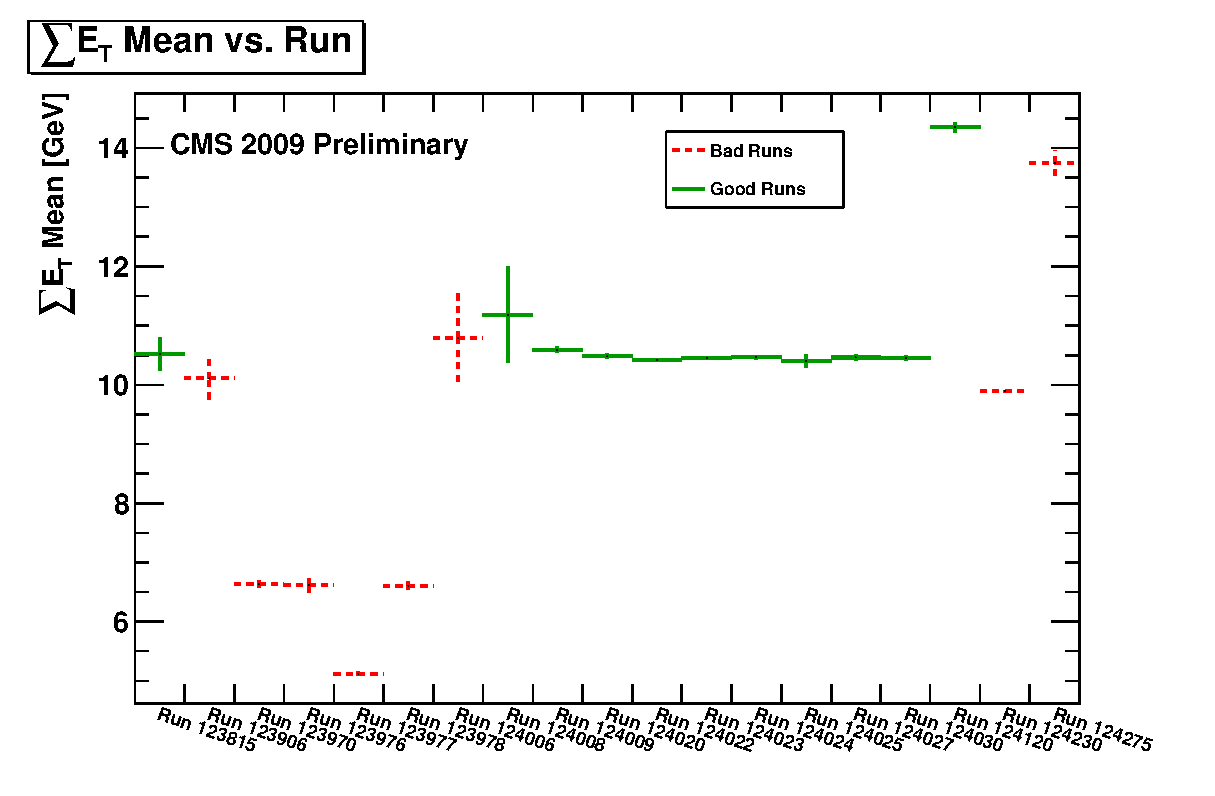
\includegraphics[width=0.5\textwidth]{plots_METStability/h_caloSumetMean_vs_run.eps} &
  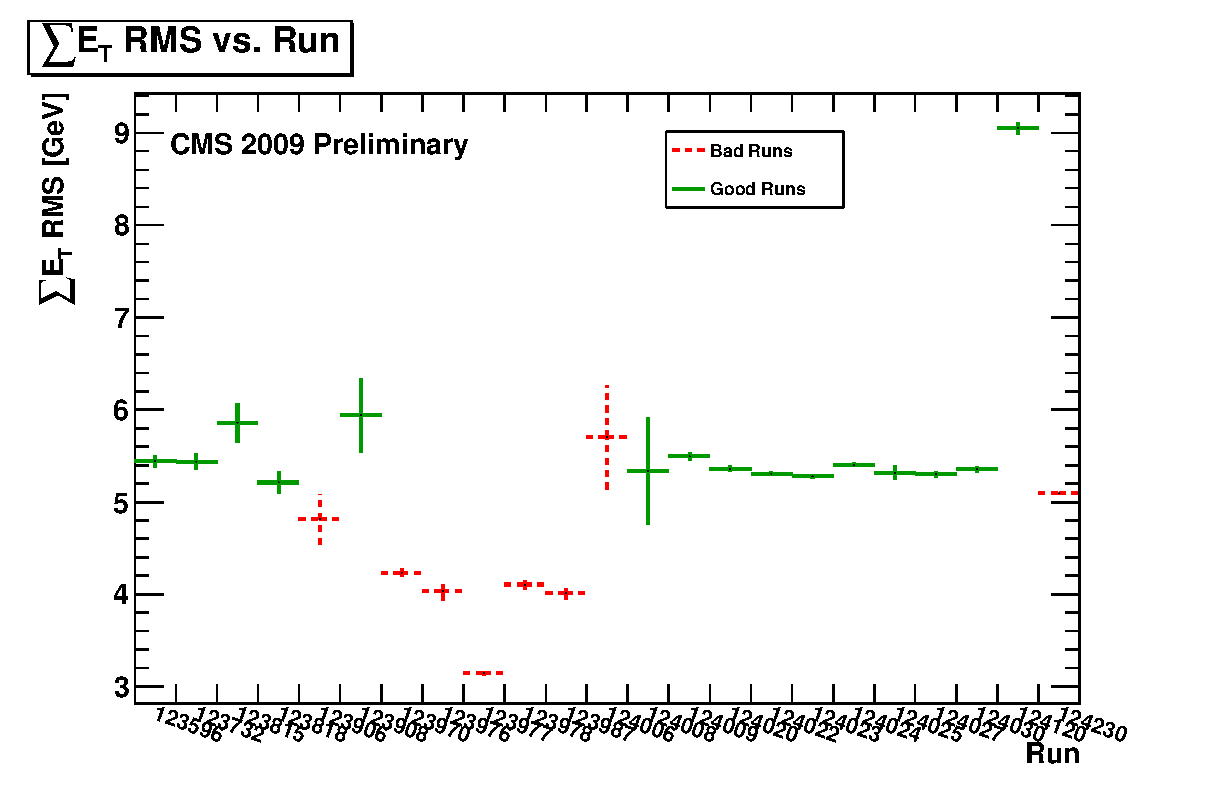
\includegraphics[width=0.5\textwidth]{plots_METStability/h_caloSumetRMS_vs_run.eps} \\
 \end{tabular}
 \caption{\small The mean and RMS of the $\sum E_\text{T}$ distribution vs. run number for the 2009 data-taking period.
          Entries shown in red correspond to runs with some known hardware problems. The last entry corresponds to a $2360$ GeV run.
          \label{fig:SumET_vs_run}}
\end{figure}

\begin{figure}[h!]
 \centering
 \begin{tabular}{ll}
  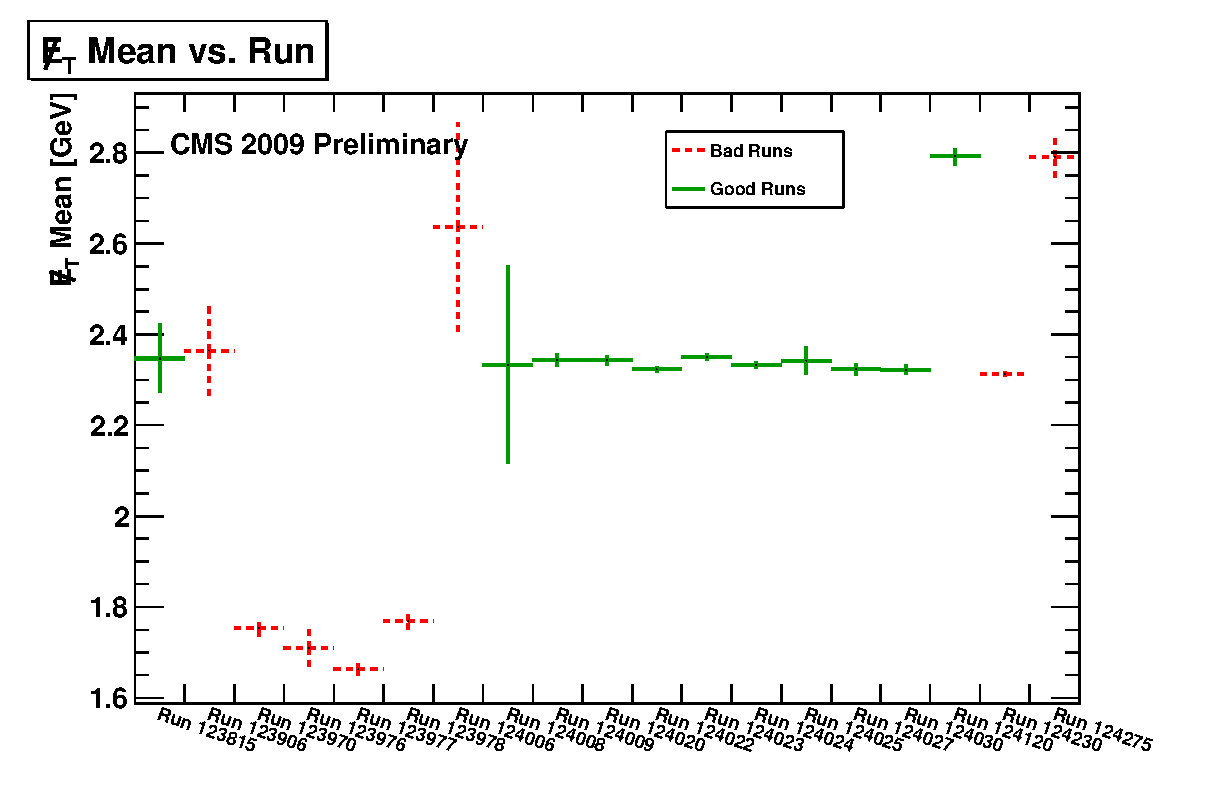
\includegraphics[width=0.5\textwidth]{plots_METStability/h_calometPtMean_vs_run.eps} &
  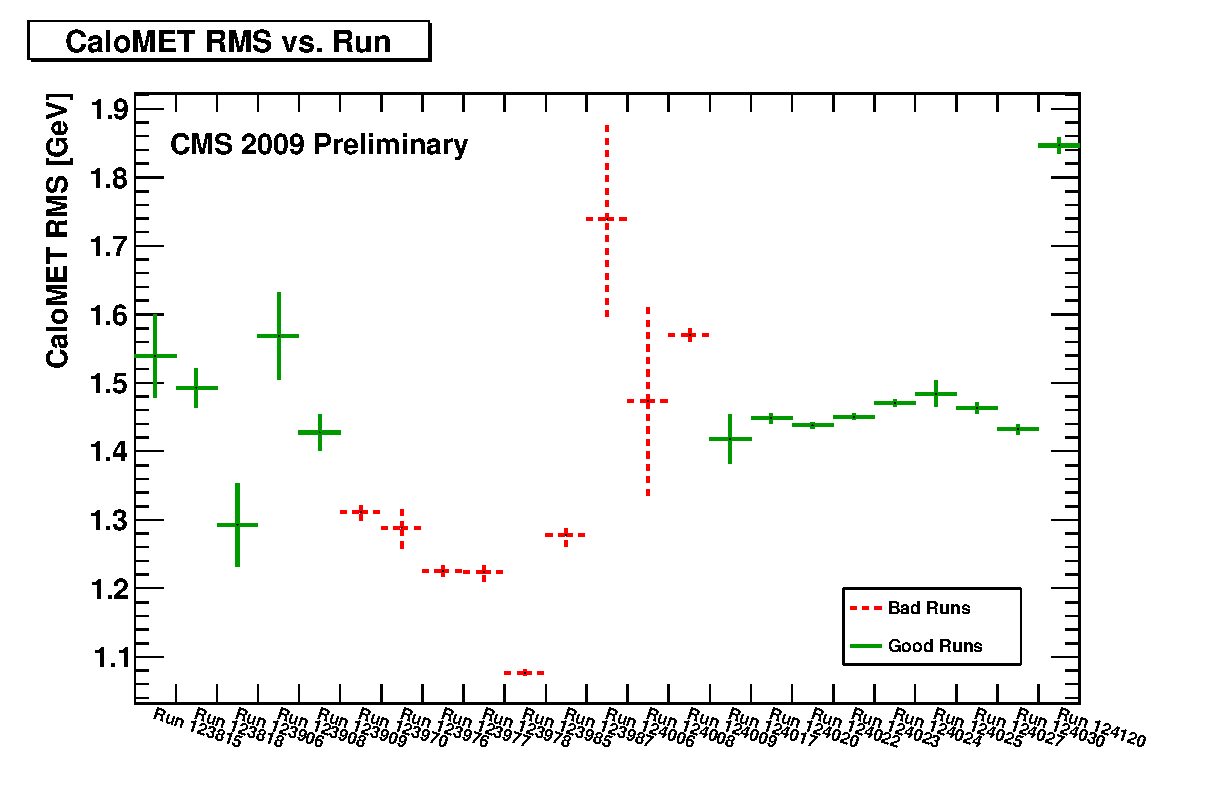
\includegraphics[width=0.5\textwidth]{plots_METStability/h_calometPtRMS_vs_run.eps} \\
 \end{tabular}
 \caption{\small The mean and RMS of the $\etmiss$ distribution vs. run number for the 2009 data-taking period.
          Entries shown in red correspond to runs with some known hardware problems. The last entry corresponds to a $2360$ GeV run.\label{fig:MET_vs_run}}
\end{figure}

\begin{figure}[h!]
 \centering
 \begin{tabular}{ll}
  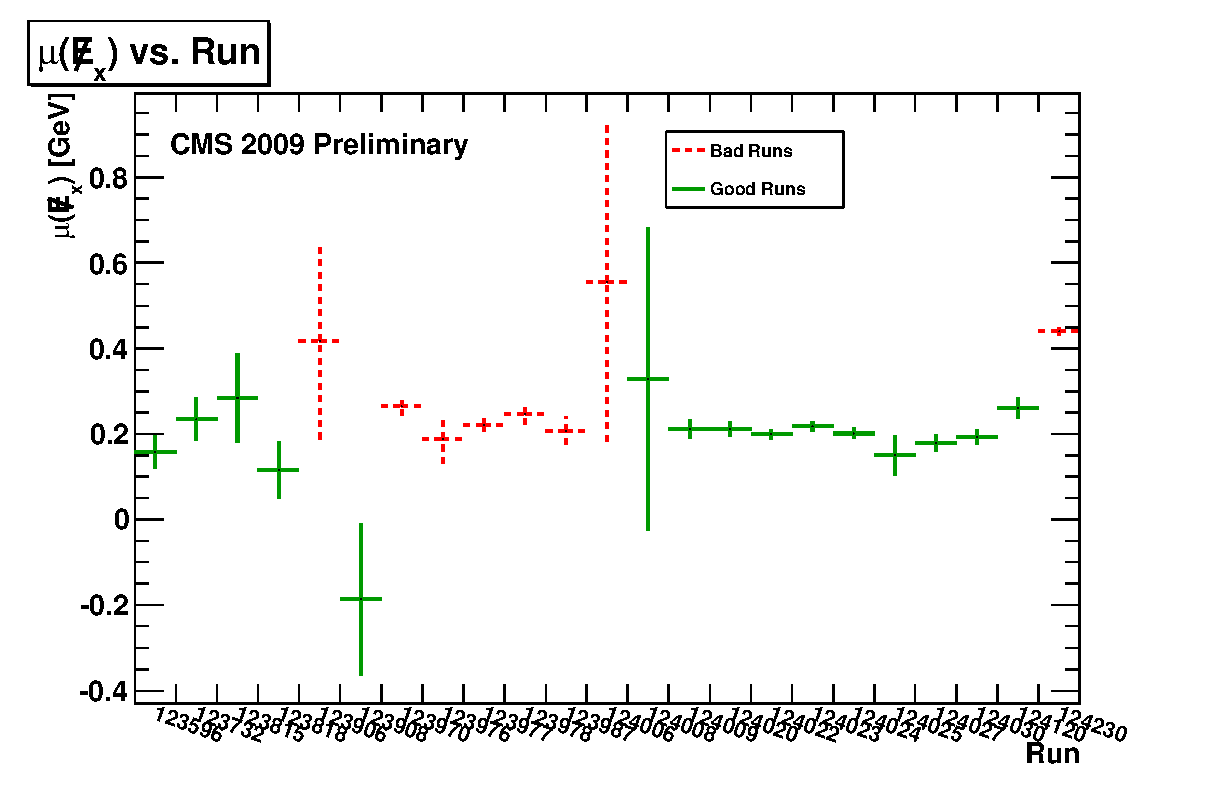
\includegraphics[width=0.5\textwidth]{plots_METStability/h_calometPxMean_vs_run.eps} &
  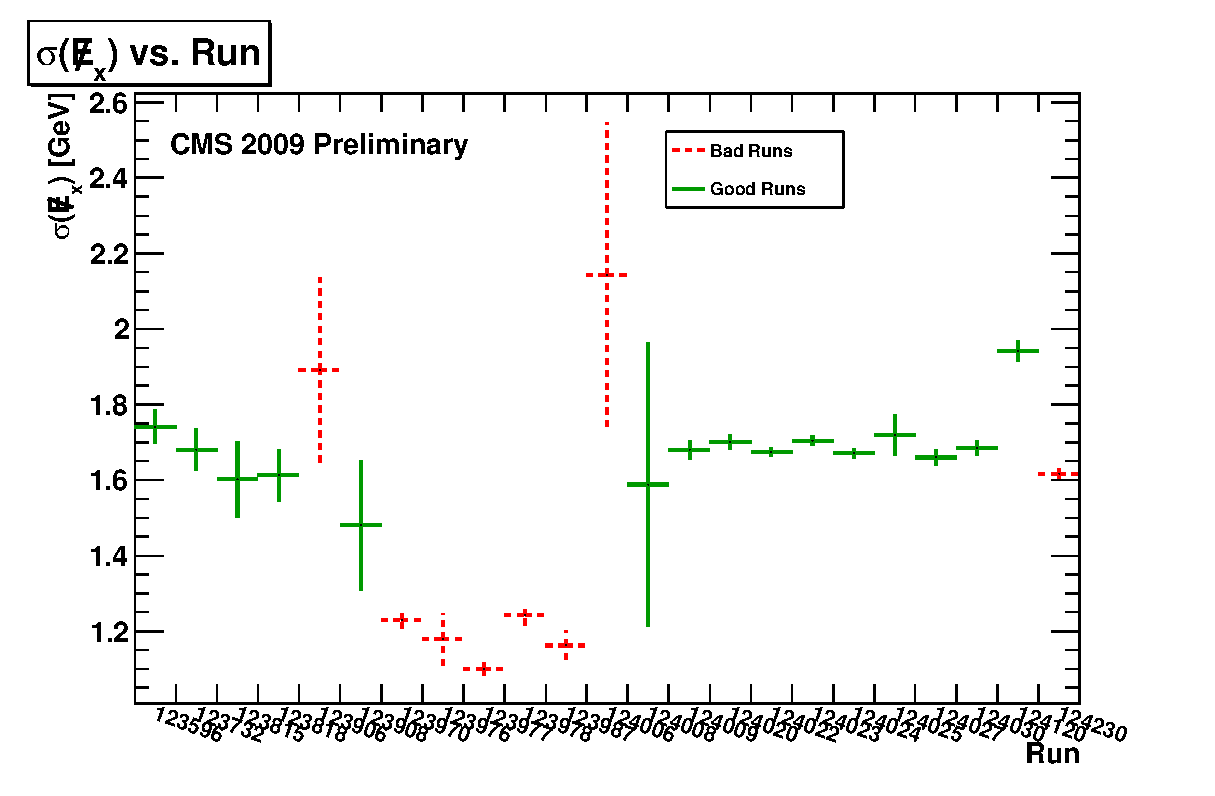
\includegraphics[width=0.5\textwidth]{plots_METStability/h_calometPxSigma_vs_run.eps} \\
 \end{tabular}
 \caption{\small The mean and $\sigma$ of the $\exmiss$ distribution vs. run number for the 2009 data-taking period.
          Entries shown in red correspond to runs with some known hardware problems. The last entry corresponds to a $2360$ GeV run.\label{fig:MEx_vs_run}}
\end{figure}

\begin{figure}[h!]
 \centering
 \begin{tabular}{ll}
  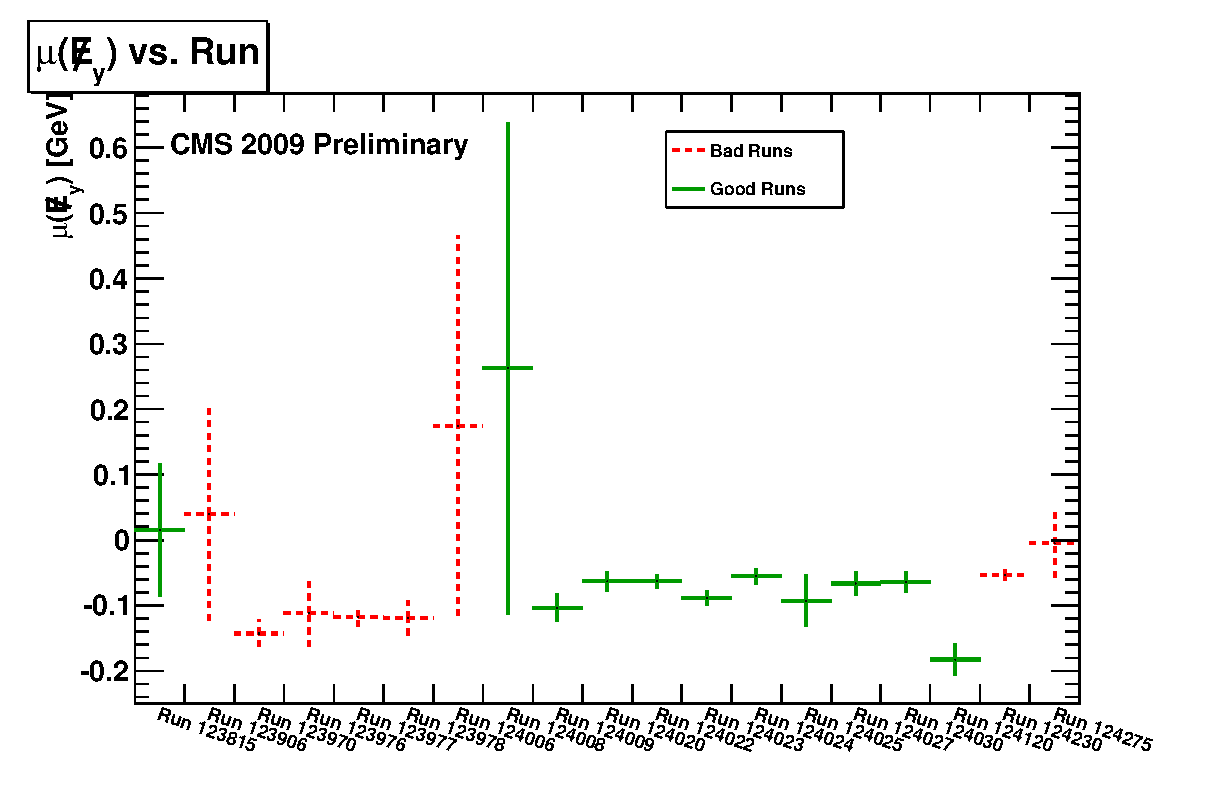
\includegraphics[width=0.5\textwidth]{plots_METStability/h_calometPyMean_vs_run.eps} &
  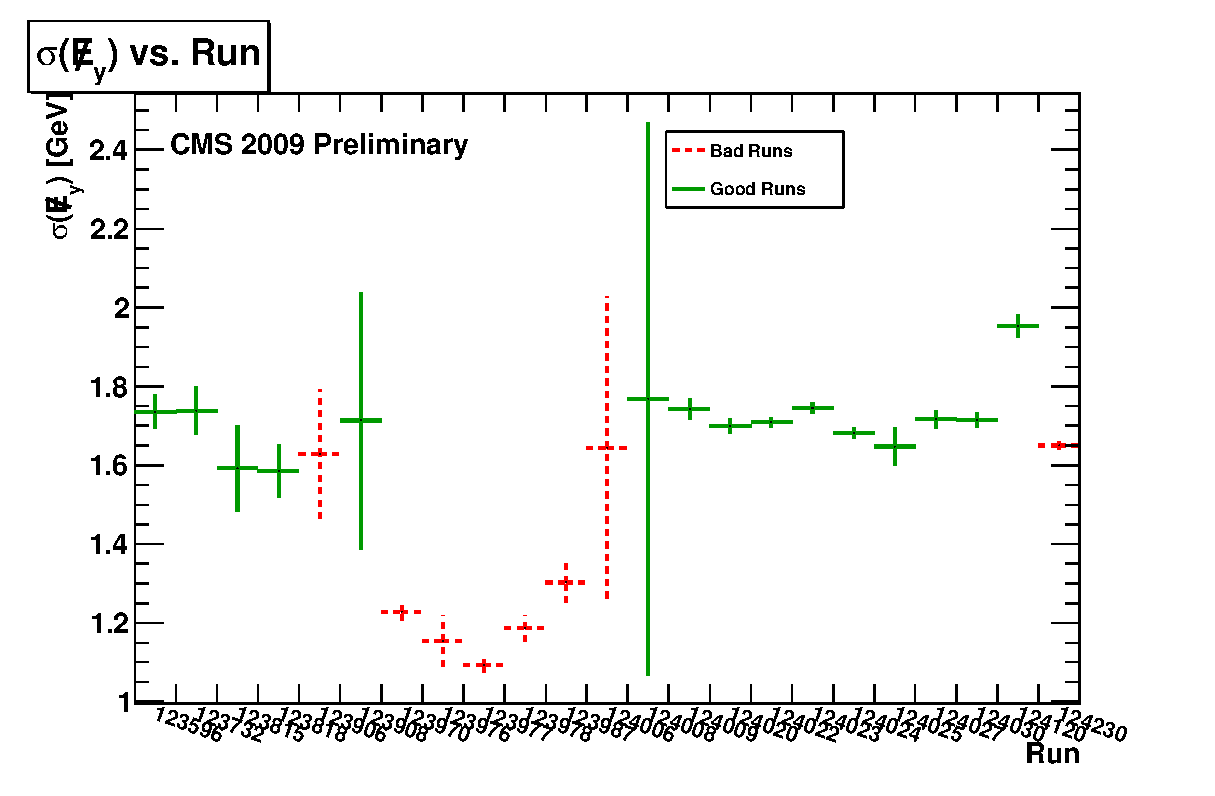
\includegraphics[width=0.5\textwidth]{plots_METStability/h_calometPySigma_vs_run.eps} \\
 \end{tabular}
 \caption{\small The mean and $\sigma$ of the $\eymiss$ distribution vs. run number for the 2009 data-taking period.
          Entries shown in red correspond to runs with some known hardware problems. The last entry corresponds to a $2360$ GeV run.\label{fig:MEy_vs_run}}
\end{figure}


\clearpage

